%%% template.tex
%%%
%%% This LaTeX source document can be used as the basis for your technical
%%% paper or abstract. Intentionally stripped of annotation, the parameters
%%% and commands should be adjusted for your particular paper - title, 
%%% author, article DOI, etc.
%%% The accompanying ``template.annotated.tex'' provides copious annotation
%%% for the commands and parameters found in the source document. (The code
%%% is identical in ``template.tex'' and ``template.annotated.tex.'')

%\documentclass[annual]{acmsiggraph}
\documentclass[review]{acmsiggraph}            

\usepackage{subfigure}

%% The 'graphicx' package allows for the inclusion of EPS figures.

\usepackage{graphicx}

%% use this for zero \parindent and non-zero \parskip, intelligently.

\usepackage{parskip}

%% Optional: the 'caption' package provides a nicer-looking replacement
%% for the standard caption environment. With 'labelfont=bf,'textfont=it',
%% caption labels are bold and caption text is italic.

\usepackage[labelfont=bf,textfont=it]{caption}

%% If you are submitting a paper to the annual conference, please replace
%% the value ``0'' below with the numeric value of your OnlineID.
%% If you are not submitting this paper to the annual conference,
%% you may safely leave it at ``0'' -- it will not be included in the output.

\usepackage{color}

\graphicspath{{images/}}

%% paper: 1046
\TOGonlineid{1046}
\TOGvolume{0}
\TOGnumber{0}
\TOGarticleDOI{1111111.2222222}
\TOGprojectURL{}
\TOGvideoURL{}
\TOGdataURL{}
\TOGcodeURL{}

\title{Project PAALM: Phalangeal Angle Approximation through the Leap Motion Controller}

\author{Michael L. Rivera\thanks{e-mail:mrivera.lee@gmail.com}\\University of Pennsylvania}
\author{Aline Normoyle\thanks{e-mail:alinen@seas.upenn.edu}\\University of Pennsylvania}
\author{Normal I. Badler\thanks{e-mail:badler@seas.upenn.edu}\\University of Pennsylvania}
\pdfauthor{Aline Normoyle}

\keywords{user interfaces,motion capture,hand animation}

\begin{document}

%% \teaser{
%%   \includegraphics[height=1.5in]{images/sampleteaser}
%%   \caption{Spring Training 2009, Peoria, AZ.}
%% }

\teaser{
\centering
\subfigure[]{
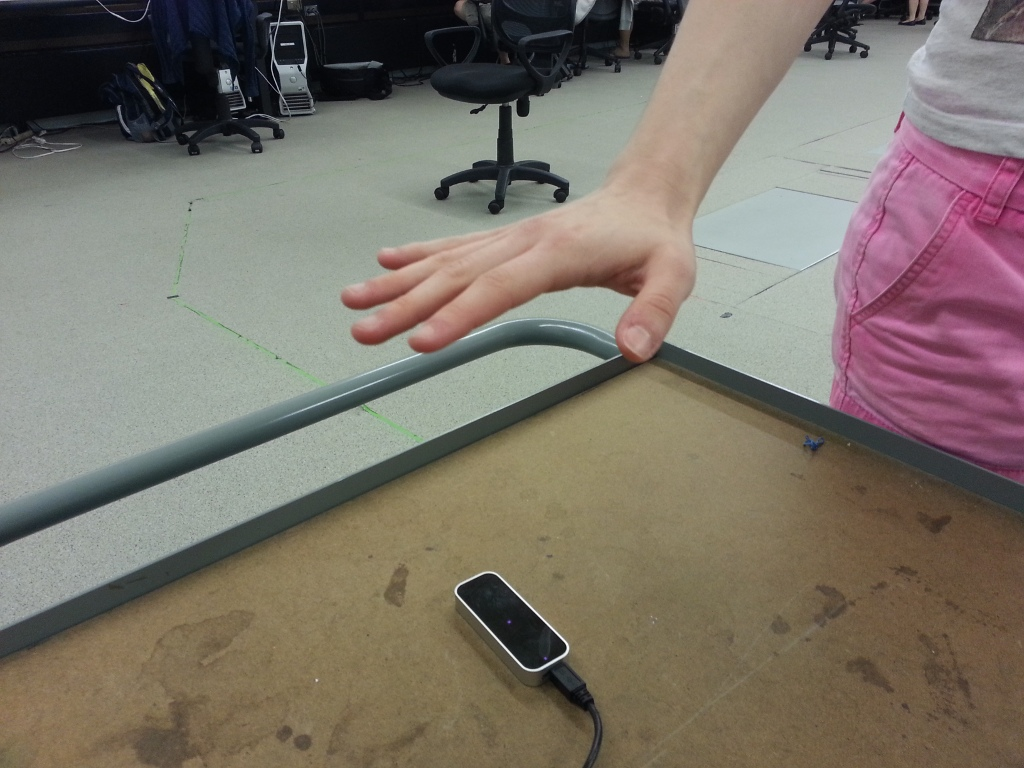
\includegraphics[scale = 0.1]{hand-input-01.jpg}
\label{fig:Video1}
}
\subfigure[]{
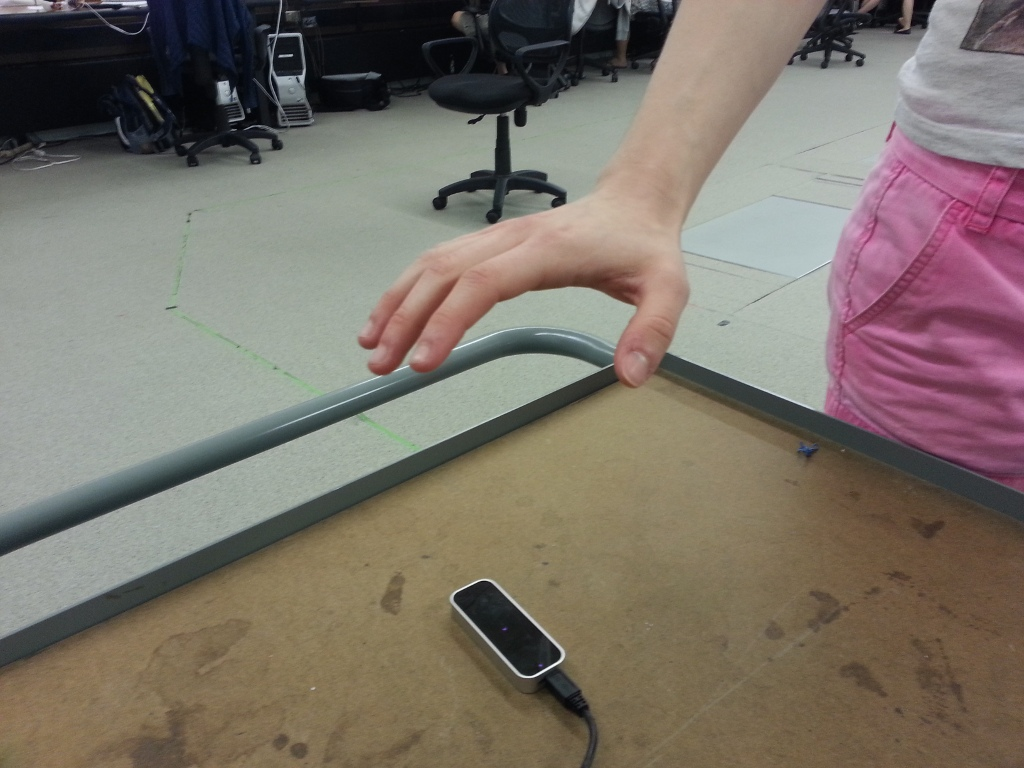
\includegraphics[scale = 0.1]{hand-input-02.jpg}
\label{fig:Video2}
}
\subfigure[]{
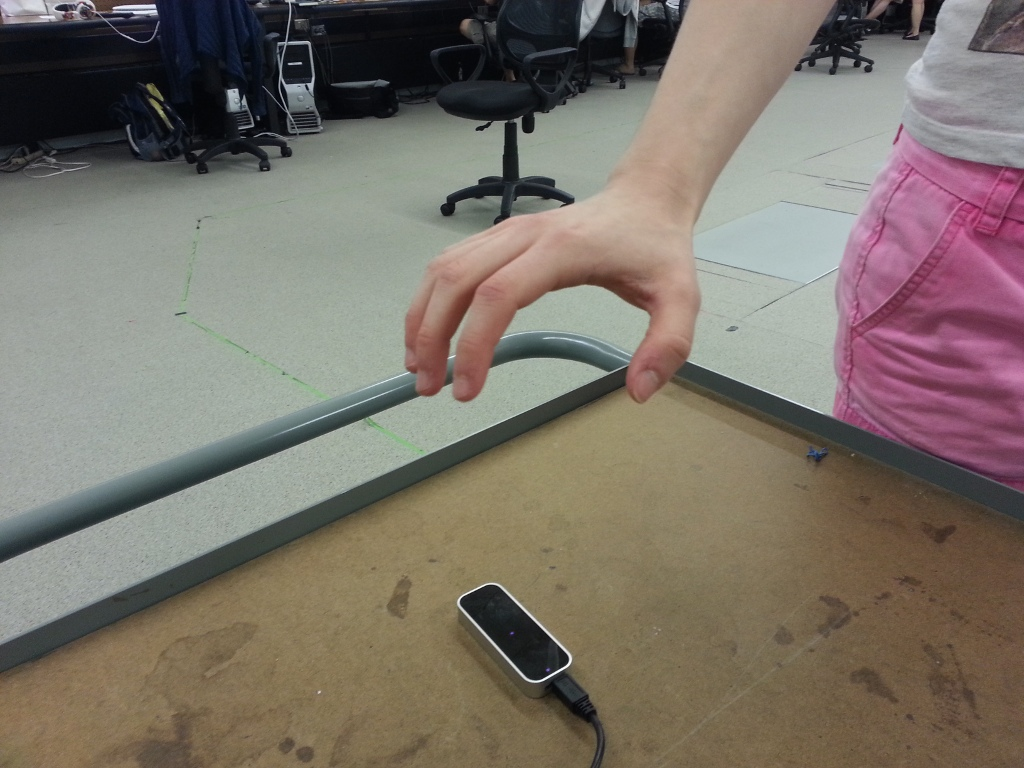
\includegraphics[scale = 0.1]{hand-input-03.jpg}
\label{fig:Video3}
}
\subfigure[]{
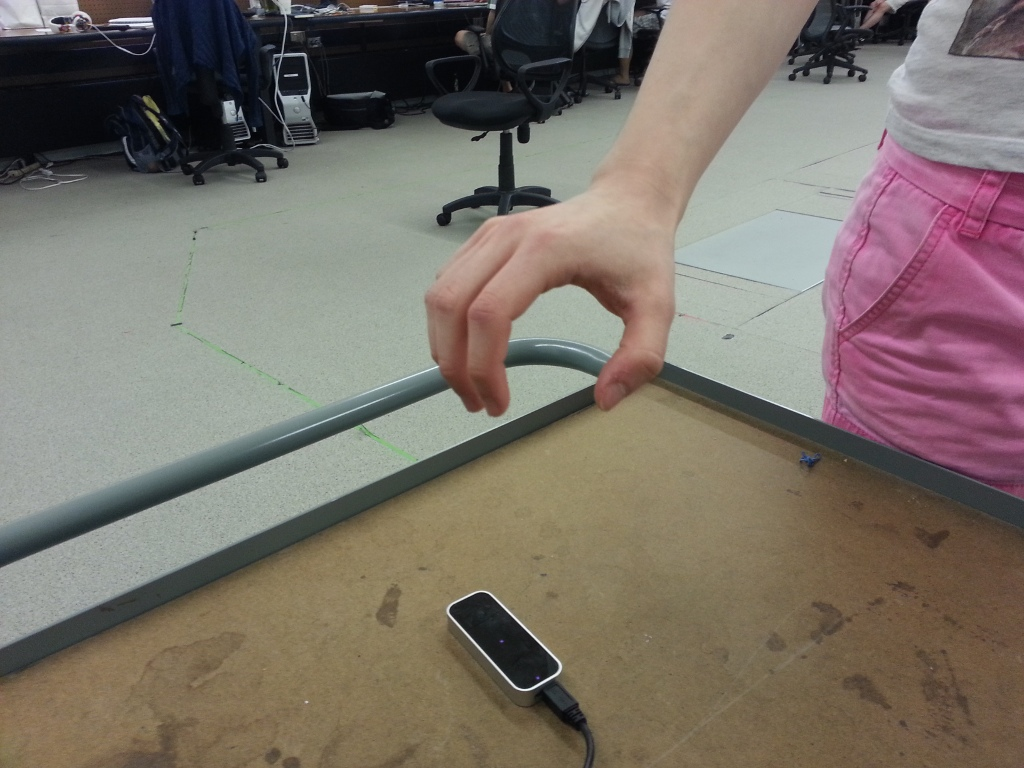
\includegraphics[scale = 0.1]{hand-input-04.jpg}
\label{fig:Video4}
}
\subfigure[]{
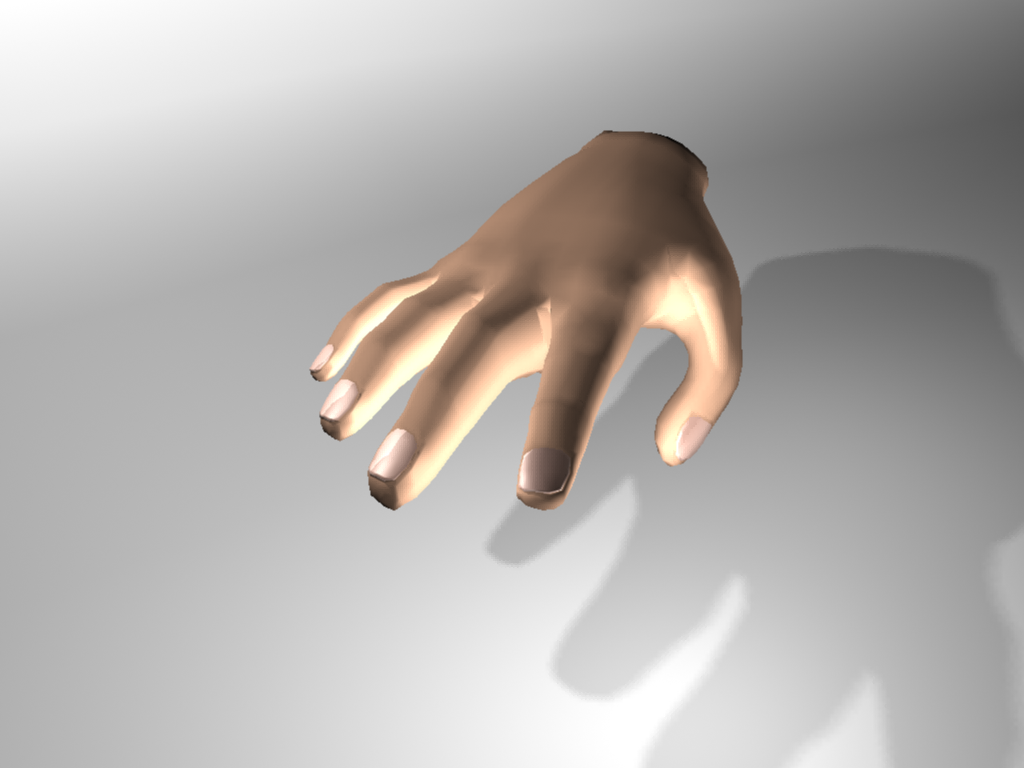
\includegraphics[scale = 0.1]{hand-rendered-01.png}
\label{fig:Maya1}
}
\subfigure[]{
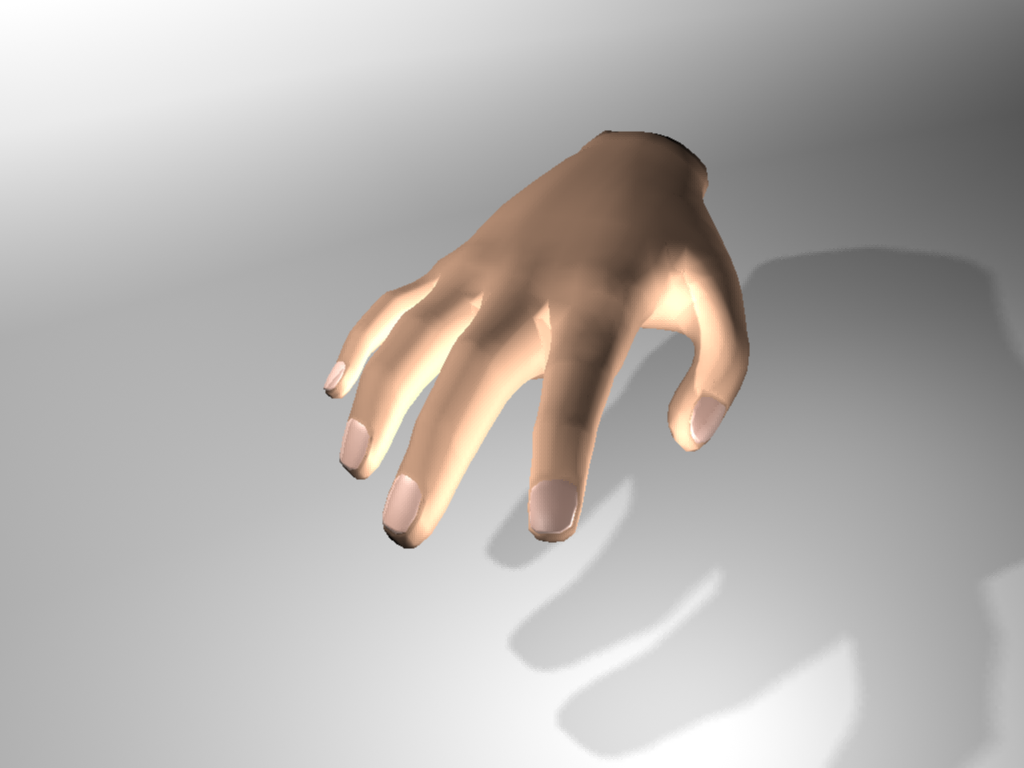
\includegraphics[scale = 0.1]{hand-rendered-02.png}
\label{fig:Maya2}
}
\subfigure[]{
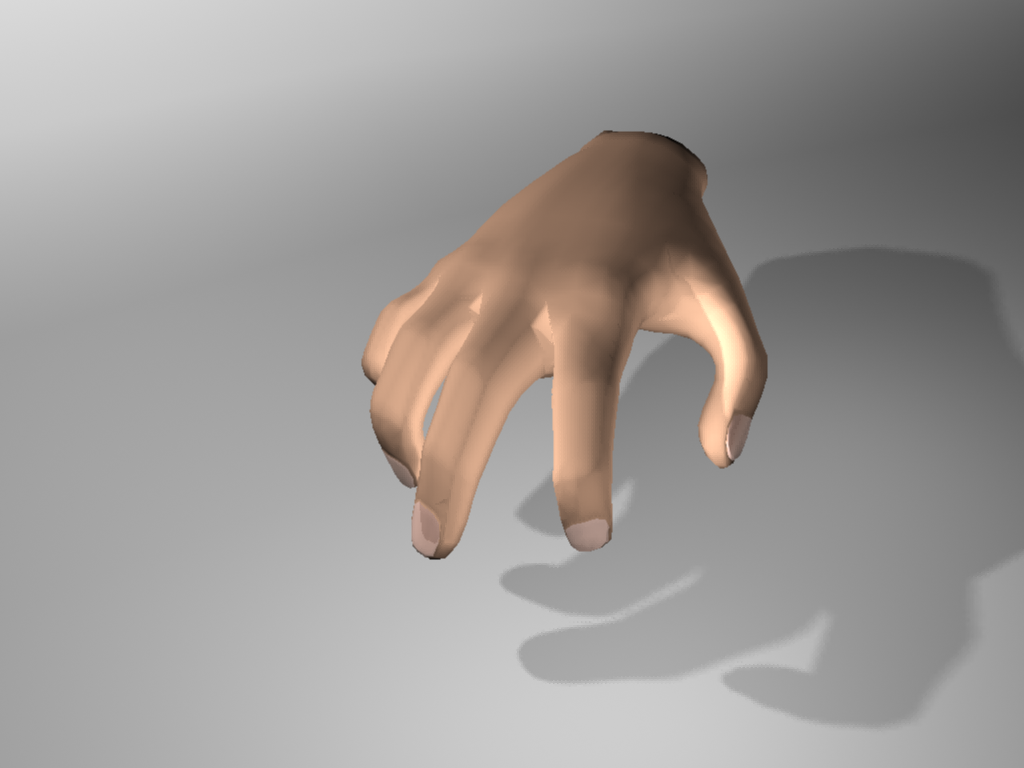
\includegraphics[scale = 0.1]{hand-rendered-03.png}
\label{fig:Maya3}
}
\subfigure[]{
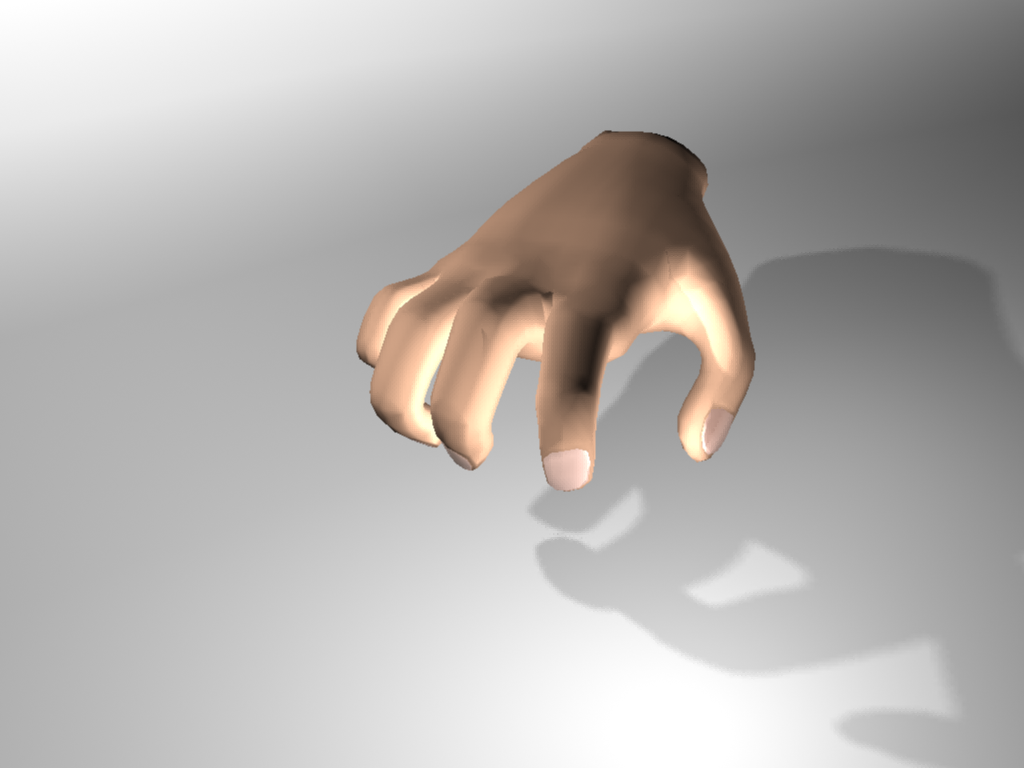
\includegraphics[scale = 0.1]{hand-rendered-04.png}
\label{fig:Maya4}
}
\vspace{-0.3cm}
\caption{Top Left to Right: The Leap Motion controller tracks to palm and fingers above it. 
Bottom Left to Right: Our PAALM system estimates finger positions in real-time based on the Leap input. 
The bottom animation was created using a Maya plugin which communicates directly with the device to 
create keyframes for a hand model.}
\vspace{-0.5cm}
}



\maketitle

\begin{abstract}

Hands are fundamental in a variety of domains including 
character animation, sign language, robotics, and 
gestural user interfaces. However, the dexterity and
flexibility of the hand make it difficult to accurately capture
information about complex gestures. Current approaches
are expensive, restrict movement of the hand, confine the
user to a capture region, or require time-consuming manual 
cleanup. Thus, we investigate the use of a fast, approximate, 
and inexpensive method for obtaining the phalangeal joint 
angles of the hand using the Leap Motion Controller~\cite{LEA}. 
Our framework directly integrates the Leap Motion controller 
into Maya to create an intuitive user interface for animating hand motions.

\end{abstract}

% TODO
\begin{CRcatlist}
  \CRcat{I.3.3}{Computer Graphics}{Three-Dimensional Graphics and Realism}{}
  \CRcat{I.3.7}{Computer Graphics}{Three-Dimensional Graphics and Realism}{};
\end{CRcatlist}

\keywordlist

\TOGlinkslist

\copyrightspace

\section{Introduction}

Hands are fundamental in a variety of domains including 
character animation, sign language, robotics, and 
gestural user interfaces. Hands are both the 
primary mechanism we use to interface with the physical
world as well as an important component for communication. 
In computer graphics, the realistic animation of the
human hand is a long-standing and difficult  problem 
because our hands are very dexterous and versatile.
Detailed and subtle finger motions are important for 
lifelike characters but are difficult to capture.
Much research has been devoted to efficiently 
capturing hand gestures, using imaged-based, glove-based, 
and marker-based techniques. However, most existing methods remain
expensive, can restrict the motion of the hand, might confine the user to a
space, or require time-consuming manual cleanup.
For example, dexterous finger motions are very difficult to capture with 
optical and marker-based systems because markers frequently 
become occluded and the proximity of the fingers cause automatic 
labeling algorithms to frequently mislabel markers.  Conversely, solutions 
involving wearable measurement devices, such as cybergloves, are 
often bulky and restrict delicate movements. 

We use the data from the Leap controller to estimate the phalangeal 
joint angles of the fingers and palm. 
Thus, we investigate an effective method for approximating and recording 
hand motions that is portable, unrestrictive, real-time 
and cost-effective. Our approach utilizes a new and
unexplored technology called the Leap Motion Controller
that is roughly the size of a flash drive and tracks individual
finger movements to 1/100th of a millimeter~\cite{LEA}. This device is 
designed to sit on a desk and plugged into a PC via USB. Internally, the 
device tracks finger motions in a one meter hemispherical area above the device 
using two light sensors and three infrared LEDs ~\cite{LeapDev}. 

Our framework implements an application programming interface (API)
for obtaining and visualizing the phalangeal joint angle data
using the Leap Motion Controller which is suitable for direct import 
(via a plug-in) into a rigged Maya hand model.  Unlike a purely image-based system, 
the Leap Motion device provides users with direction vectors and lengths for 
each finger as well as an orientation and position for the palm. We map the output 
from the Leap Motion controller to IK targets for each finger based on a simple 
calibration step.

Our main contributions are as follows:
\begin{itemize}
\item An portable, cost-effective, real-time, and freehand
method of obtaining phalangeal joint angles using an
unexplored technology.
\item An application programming interface (API) for 
obtaining and visualizing the phalangeal joint angle data
using the Leap Motion Controller which is suitable for direct import 
(via a plug-in) into a rigged Maya hand model.
\end{itemize}

\section{Related Work}

Recording hands remains a difficult problem. Below we briefly outline four major approaches.

%Hanke, T. (2004), “HamNoSys - representing sign language data in language resources and language processing contexts.” In: Streiter, Oliver, Vettori, Chiara (eds): LREC 2004, Workshop proceedings : Representation and processing of sign languages. Paris : ELRA, 2004, - pp. 1-6.
%
%Vogler, C.and D. Metaxas, Handshapes and movements: multiple-channel American Sign Language recognition. In A. Camurri and G. Volpe (eds.), Gesture-Based Communication in Human-Computer Interaction, 5th International Gesture Workshop, GW 2003, Genova, Italy, April 15-17, 2003, Selected Revised Papers. Berlin: Springer. 247-258.


\subsection{Marker-based Systems}

Marker-based motion capture systems are a popular
means of obtaining hand motion data. The standard approach
requires attaching approximately 30 retro-reflective
markers to the hand and tracking them over time ~\cite{VIC}.
The temporal data is then used to reconstruct a 3D representation
of the hand and its motions.
Recent advancements in hand motion capture have made
it possible to achieve descriptive hand motion data with a
reduction in the number of markers ~\cite{HRM12}. Though
even with such advancements, marker-based approaches
still pose significant problems in hand motion detection.
Gestures featuring self-occlusion (fingers overlapping one
another) are difficult to detect using the system. Automatic
marker tracking is not effective in maintaining the markers
over time. Thus, the process of tracking markers is then a
tedious one, requiring manual labeling that is both time-consuming
and error prone ~\cite{ZCX12}.


\subsection{Glove-based Systems}

Glove-based systems such as the CyberGlove ~\cite{CYB}
provide a useful method of obtaining hand gesture data that
is free from issues that arise when fingers occlude each
other. Such systems have been used for the recognition of 
sign language~\cite{Vogler03Handshapes}. 
The motions recorded using the system, however, are
often noisy and fail to capture delicate articulations with
high precision ~\cite{ZCX12}. Likewise, the system restricts the
natural motion of the hand, making capturing realistic gestures
a more complex task. The advantage of using the
Leap Motion Controller for our approach is that it permits
the hand to move freely and naturally. 

\subsection{Image-based Systems}

Computer vision has offered a promising alternative to
data gloves and other worn mechanisms for detecting hand
motions ~\cite{EBN07}. Image-based systems have the advantage 
of being lower cost, portal, and not restrictive of hand movements.

Image-based approaches must handle occlusions between fingers. 
~\cite{LaGorce11ModelBased} tracked hand poses based on 
monocular video using a model of temporal continuity to handle occlusions. 
Other image-based techniques rely on hand motion priors stored in a large 
database to aid capture ~\cite{Wu01CapturingHand,Zhou03TrackingHand,Wang09ColorGlove,Romero10Hands}. 
However, these approaches rely on having a large hand database to guide pose 
recognition and generation and thus have the drawbacks of requiring 
a large number of pre-collected poses and thus whose recognition is 
restricted to poses similar to those in the database. 
In an other approach, ~\cite{Oikonomidis11EfficientModel} enhanced 
the accuracy of imaged-based techniques through the use of a RGB-depth camera. 
A recent device called Digits has been developed that
uses a wrist-worn gloveless sensor to detect 3D hand gestures
~\cite{KHI12}. The sensor features two infrared illumination
schemes that are used to produce a hand model
through inverse kinematics. The wrist-worn device avoids
the need for any embedded sensors in the environment and
permits the hand to move freely as well as the user to move
about without being confined to a capturing region.
Vision-based techniques have the drawbacks of being computationally expensive, 
noisy and vunerable to a lack of obvious features on the hand and occlusions.

\subsection{Hybrid Systems}

A recent innovation has been combining marker-based
and image-based systems to provide higher fidelity hand
motion data ~\cite{ZCX12}. These systems are capable of accurately
detecting hand motions even in cases of selfocclusion.
The markers are used as reference when rebuilding
hand motion data using an RGB-depth camera such as
the Microsoft Kinect. These systems are robust and do not
significantly restrict hand movements as the markers are
small. The potential shortcomings of this system is that it still requires 
an expensive, non-portable optical motion capture system to 
capture the markers and must run a computationally 
expensive optimization to solve for hand positions which 
saistify both the RGB-D image and the marker positions. 

\section{LEAP}

The Leap Motion Controller offers a cost-effective, fast
and precise means of capturing live hand motion data.
This device is small (3x1x0.5 inches), 
designed to sit on a desk and plugged into a PC via USB. Thus, it is 
extremely portable and lightweight. 

\begin{figure}
\centering
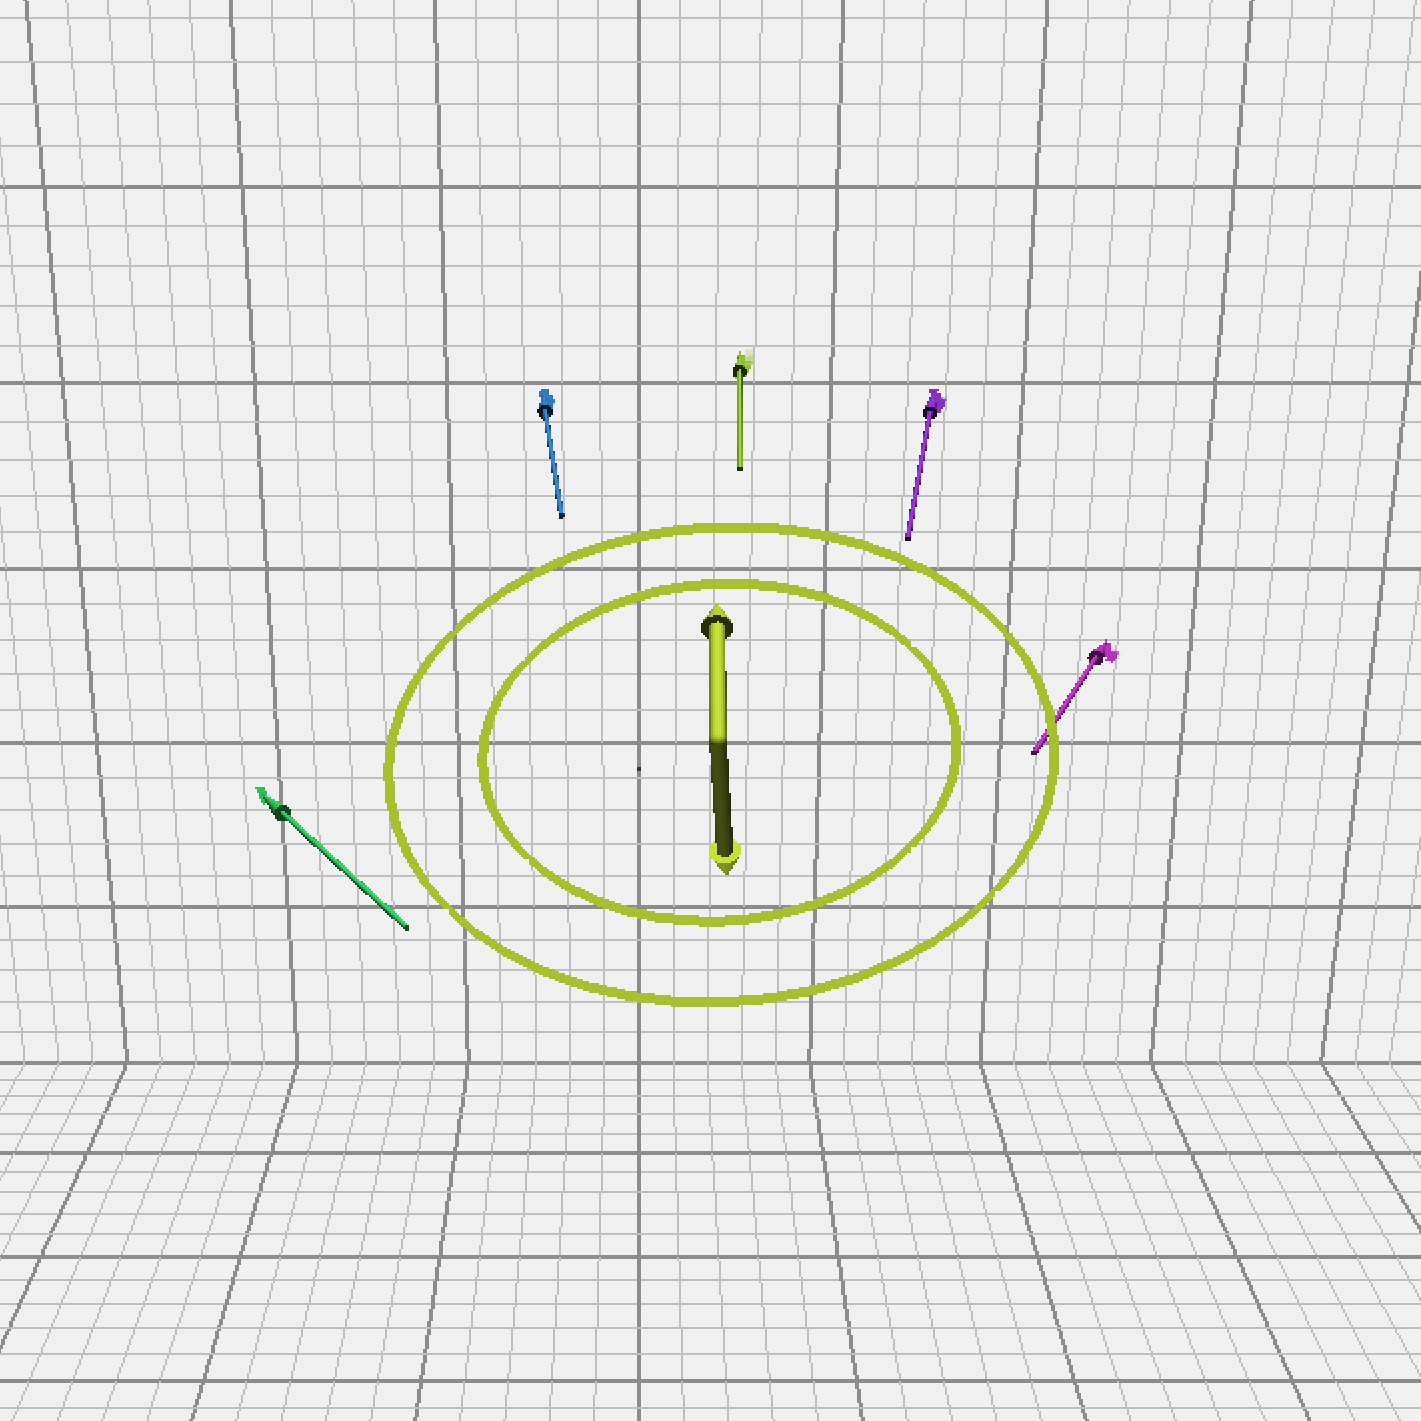
\includegraphics[scale=0.27]{leap-palm-and-fingers.png}
\vspace{-0.1cm}
\caption{Leap Motion visualizer displaying finger vectors and a palm normal for a hand. \label{LeapUI}}
\vspace{-0.5cm}
\end{figure}

\begin{figure}
\centering
\subfigure[]{
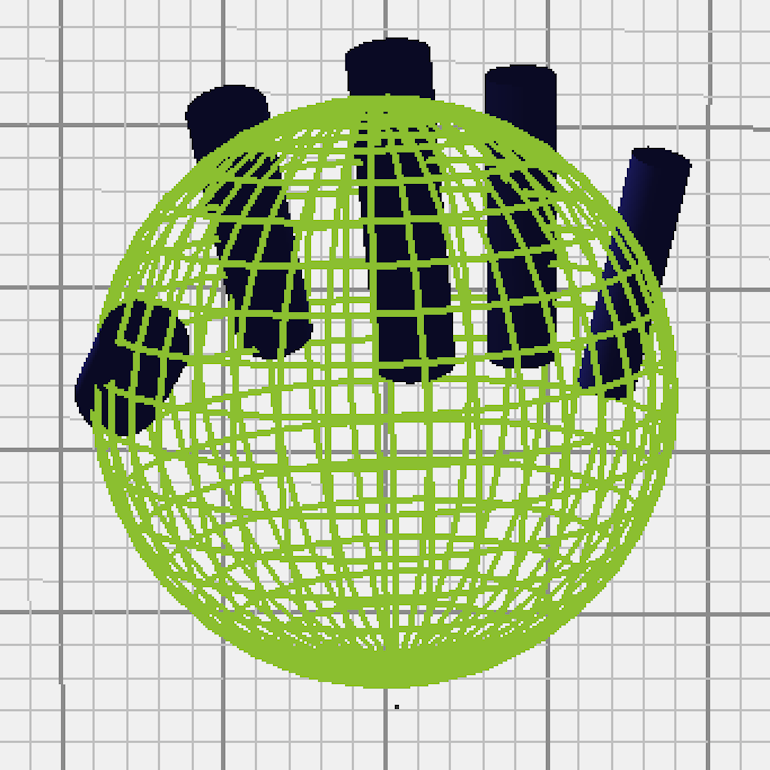
\includegraphics[scale=0.13]{palm_small_radius.png}
\label{fig:Palm1}
}
\subfigure[]{
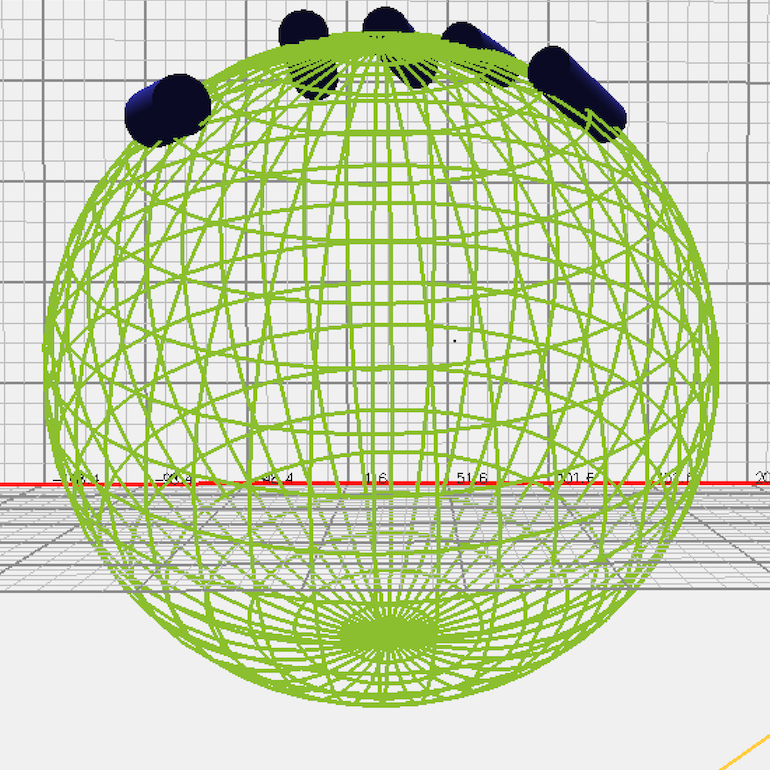
\includegraphics[scale=0.13]{palm_large_radius.png}
\label{fig:Palm1}
}
\vspace{-0.1cm}
\caption{Top to Bottom: Leap Motion visualizer displaying the palm radius
 for a partially closed hand and an open hand with spread fingers.\label{Palm}}
\vspace{-0.5cm}
\end{figure}

The Leap Motion Controller is an infrared-based device, featuring three infrared 
LEDs and two light sensors. The device is capable of tracking position changes as 
small as a 1/100th of a millimeter within a detection region of eight cubic feet. Its 
sensors capture spatial information at 290 frames per second and provide data 
about the tip position, tip velocity, length, direction, and width of pointable objects, 
such as a pen or a finger, in 3D space. 

With respect to fingers, the device can determine to which hand a set of fingers 
belong and provide details about a hand's palm position and normal (Figure~\ref{LeapUI}). 
Additionally, the hand data includes a palm sphere radius, or the radius of a spherical
 object that could be held within the palm of the hand. A small radius suggests a closed 
hand while a large radius suggests an open hand with fingers spread further apart (Figure~\ref{Palm}).  
Occluded fingers are not detected by the device, so crossed or folded fingers will 
disappear from the output data until they are detected again.

All of the data provided by the Leap Motion Controller is organized into individual 
frames which can be accessed and manipulated using the device's application programming interface.

%The Leap Motion Controller is not currently available to the general public. We were able to obtain a developer release of the controller through an application process available on the Leap Motion web site.  An official release date for the device has been set for May 13, 2013. The cost of the device will be  \$79.99. 

\section{Approach}

\begin{figure}
\centering
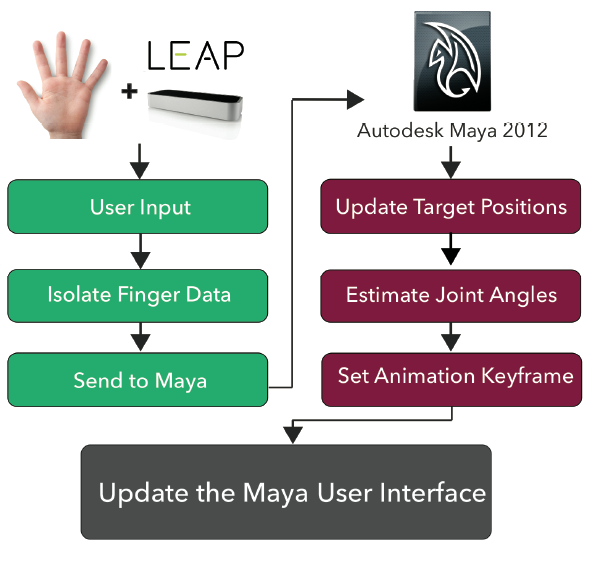
\includegraphics[scale=0.4]{Overview.png}
\vspace{-0.3cm}
\caption{PAALM Overview. To isloate finger data, we sort detected fingers by x-ccordinate and compute 
a ratio for estimating the amount of bend in the finger. This data is sent to a Maya plugin via a socket, 
occurring through Maya's command port. 
We then compute IK target positions by computing an offset for the finger tip based on a direction 
vector offset from the first knuckle joint of each finger. Finally, we set keyframes which may then be 
rendered out or exported to a motion file format.\label{HighLevel}}
\vspace{-0.5cm}
\end{figure}

In this section, we describe how we map the output from the Leap device to a joint hierachy 
in Maya.  The device API provides unordered direction vectors whose lengths 
correspond to the length of each finger seen by the device. The device omits information 
for any fingers it fails to detect, such as fingers folded into the palm or crossed together.
The size, position, and orientation of the palm is also provided by the Leap API. 

Thus, inferring hand positions from the Leap input requires mapping these direction 
vectors to the finger and palm of our model. 

For this straighforward approach to work, we must first calibrate our system for 
the finger sizes of the capture subject, which can differ greatly between individuals. 
During this step, our capture subject need only 
hold their hand above the leap device in a rest pose with open palm and spread 
fingers, such that the device can detect the entire hand.  We then record  
lengths of each finger over 1000 frames (approximately 10 seconds) and use the average 
as the standard length $\ell_s$ for the finger. The standard length is then compared against the 
current length $\ell_c$ in all subsequently captured frames to compute a length ratio $\frac{\ell_c}{\ell_s}$.

In Maya, we define joint chains for each finger apriori (which we will designate 
as Maya-fingers)  having joint limits and sensible degree of freedom constraints. The leap direction 
vectors $d$ are then scaled based on the length of each Maya-finger $\ell_m$ and the leap finger ratio to 
compute an offset from first knuckle of each Maya finger. 
\[
x_{ik} = \ell_m \frac{\ell_c}{\ell_s} \frac{d}{||d||} + x_{knuckle}
\]
where $x_{ik}$ is the global position for placing our IK target and $x_{knuckle}$ is the global 
position of the knuckle. Each frames, we then update the finger positions based on IK. Each N frames, 
we additionally save out a keyframe, with N chosen to based on the desired framework of the animation.
These keyframes can either be rendered out as is, or exported to a 
standard motion format, such as amc/asf, v/vsk, or bvh.

Lastly, we must account for two complicating factors: one, the finger data for a hand 
received from the Leap Motion Controller is not guaranteed to be ordered; and two, some 
number of fingers might not be detected at all. The first problem is solved with a heuristic where 
we sort the finger data by x-coordinates in 3D space (chosen because it matches the orientation of a detected
hand in the device's coordinate space). In our demos, we us ethe right hand although the system is 
suitable for either hand or can support two hands if they are not stacked on top of each other.
The configuration need only be specified during calibration. 
The sorted fingers receive unique identifiers that are used to associate  
 standard lengths (acquired during calibration) with lengths from subsequent frame updates. 
We deal with the second problem using heuristics to infer the missing finger, e.g. 
we assume that a finger will stay in the same position until it is detected again.

Our implementation has two main components: a Python script for interfacing with the 
Leap Motion Controller and a Maya plug-in written in PyMel for animating hand motions.
The integration between the Leap controller and our Maya plug-in is socket-based, 
occurring through Maya's command port. 


%\begin{equation}
% \sum_{j=1}^{z} j = \frac{z(z+1)}{2}
%\end{equation}
%
%\begin{eqnarray}
%x & \ll & y_{1} + \cdots + y_{n} \\
%  & \leq & z
%\end{eqnarray}

\section{Conclusion}

This work describes a simple, straight forward mapping of the leap device for estimating hand poses. 
Our framework directly integrates the Leap Motion controller into Maya to create an intuitive user
 interface for animating hand motions, but could be used as well as for puppeteering other rigged models.
 Once animated, the poses are easily exported from maya into standard motion formats such 
as amc/asf, v/vsk, or bvh.

The Leap Motion controller shows much promise for the collection of hand gestures, thanks to its 
small size, cost, and input capabilities which are tuned to the detection of hands. 

The downsides of our current implementation is that it does not deal with the small levels of 
noise which are sometimes generated by the device, nor do we yet handle enough postures robustly.
Lastly, we do not evaluate sophisticated methods for dealing with missing finger data or handling 
a wide variety of poses. This is the natural next step. However, even our simple approach produces  
compelling and intriguing results. Our hope is that this work encourages and aids others interested in trying 
this device.

%\section*{Acknowledgements}

\bibliographystyle{acmsiggraph}
\bibliography{riverapalm}
\end{document}
